\documentclass[a4paper,12pt]{report}
\usepackage{graphicx}
\usepackage{algorithm}
\usepackage{algorithmic}
\usepackage{fancyhdr}
\usepackage{cite}
\usepackage{epsfig}
%\usepackage{ieeetran}
%\usepackage{subfigure}
% 
%\usepackage{epstopdf}
\usepackage{amsthm}
\usepackage{amsmath}
\usepackage{amsfonts}
\usepackage{verbatim}
\usepackage{setspace}
\usepackage{listings}
\usepackage{subfig}
\usepackage{psfrag}
\usepackage{multicol}
\usepackage{framed}
%\begin{comment}
\usepackage[colorlinks,breaklinks=true]{hyperref}% hyperref should be the last package to be included, and perhaps there  should be one line gap between entries of bibliography 
\hypersetup{
	hypertexnames=false,
	pdftitle={K-means Clustering Algorithm: Efficient Implementation on Graphics Processing Units},
	pdfauthor={Kunjan Aggarwal},
	pdfkeywords={},
%	bookmarksnumbered,
	pdfstartview={FitH},
	colorlinks=true,
	urlcolor=black,
	linkcolor=black,%: Color for normal internal links
	anchorcolor=black,%: Color for anchor text.
	citecolor=black,%: Color for bibliographical citations in text
	filecolor=black,%: Color for URLs which open local files
%	pagecolor=blue,%: Color for links to other pages
}%
\usepackage[all]{hypcap}
%\end{comment}

\usepackage{geometry}

\setlength{\topmargin}{-13mm}
\setlength{\headheight}{6mm}
\setlength{\headsep}{7mm}
\setlength{\textheight}{245mm}
%\setlength{\oddsidemargin}{0.37in}
\newpage
%\setlength{\evensidemargin}{0in}
\setlength{\textwidth}{150mm}
\setlength{\marginparwidth}{0.5in}
\renewcommand{\baselinestretch}{1.15}
\pagestyle{fancy}
\fancyhead{}
\fancyfoot{}
\renewcommand{\headrulewidth}{0pt}
\renewcommand{\footrulewidth}{0pt}
\setlength\fboxsep{1pt}
\setlength\fboxrule{0.25pt}
%\theoremstyle{definition}
\newtheorem{mydef}{Definition}[chapter]

\renewcommand\lstlistingname{Program}%                     default is Listing
\renewcommand\lstlistlistingname{List of Programs}%        default is Listings
\addtolength{\evensidemargin}{-.875in}
\pagenumbering{roman}
\fancyfoot[CO]{\thepage}
    
%setting for algorithm environment
\algsetup{
	linenosize=\small,
	linenodelimiter=.
}

\lstset{
language=C,                             % Code langugage
basicstyle=\small,                   % Code font, Examples: \footnotesize
keywordstyle=\bf,        				% Keywords font ('*' = uppercase)
commentstyle=\it,              			% Comments font
backgroundcolor=\color{white}, 			% Choose background color
frame=single,                             % A frame around the code
tabsize=2,                              % Default tab size
captionpos=b,                           % Caption-position = bottom
breaklines=false,                        % Automatic line breaking?
breakatwhitespace=false,                % Automatic breaks only at whitespace?
showspaces=false,                       % Dont make spaces visible
showtabs=false,                         % Dont make tabls visible
morekeywords={dim3,template,__device__,__global__},  				% CUDA specific keywords
}



\usepackage{color}
%\usepackage{ulem}

\definecolor{gray}{rgb}{0.5,0.5,0.5}
\definecolor{light-gray}{gray}{0.95}
\newcommand{\sout}[1]{}
%\newcommand{\sout}[1]{\textcolor{gray}{#1}}
\newcommand{\remSection}[1]{}
\newcommand{\add}[1]{\textcolor{blue}{#1}}
%\newcommand{\add}[1]{#1}
%\newcommand{\rem}[1]{\textcolor{red}{}}
\newcommand{\rem}[1]{\textcolor{red}{#1}}
%\newcommand{\sbrem}[1]{\textcolor{magenta}{#1}}
\newcommand{\sbrem}[1]{#1}

\newtheorem{lemma}{lemma}
\newcommand{\groupSymbol}{g} %refering single group
\newcommand{\groupFn}{\Gamma} % groupFn(v) refers to dependent-group of node v
\newcommand{\rep}{rep} %representative
\newcommand{\pseudorep}{\eta} %pseudorepresentative
\newcommand{\W}{wt}
\newcommand{\PertRange}{\Re} %range
\renewcommand{\algorithmicforall}{\textbf{for each}}
\renewcommand{\algorithmicrequire}{\textbf{Input}}
\renewcommand{\algorithmicensure}{\textbf{Output}}
%\newtheorem{mydef}{Definition}


%\renewcommand{\textfraction}{0.05}
%\renewcommand{\topfraction}{0.9}
%\renewcommand{\bottomfraction}{0.9}
\renewcommand{\floatpagefraction}{.95}

\title{Efficient Implementation of K-Means clustering algorithm on Graphic Processor Unit}

\begin{document}
\begin{doublespacing}
\thispagestyle{empty}

\begin{center}
\noindent {\bf{\Large{K-means Clustering Algorithm:}}}\\
\vspace{4mm}
\noindent {\bf{\Large{Efficient Implementation on Graphics Processing Units}}}\\

\vspace{55mm}
by\\
\vspace{5mm}
{\bf{\Large Kunjan Aggarwal}}\\
\vspace{10mm}
\emph{under the guidance of}\\
\vspace{5mm}
{\bf{\Large Prof. Mainak Chaudhuri}}\\
\vspace{25mm}

\begin{center}
\centering
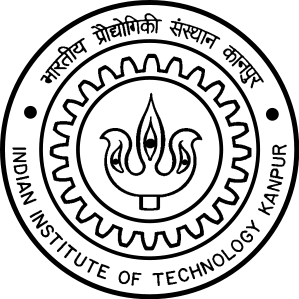
\includegraphics[width=0.25\textwidth]{./Data/iitk}
\end{center}

\vspace{3mm}
{\bf {\large {\sc DEPARTMENT OF COMPUTER SCIENCE AND ENGINEERING}}}\\
\vspace{2mm}
{\bf {\large {\sc INDIAN INSTITUTE OF TECHNOLOGY KANPUR}}}\\
\vspace{3mm}
{\textbf{ March, 2013}}\\
\end{center}


	
\newpage
\thispagestyle{empty}
\begin{singlespace}
\begin{center}
\noindent {\bf{\Large{K-means Clustering Algorithm:}}}\\
\vspace{4mm}
\noindent {\bf{\Large{Efficient Implementation on Graphics Processing Units}}}\\
\vspace{25mm}
\normalsize
\emph{A dissertation submitted in partial fulfillment} \\
\emph{of the requirements for the degree of} \\
\vspace{20pt}
\bfseries MASTER OF TECHNOLOGY \\
\vspace{10pt}
\emph {in}\\
\vspace{10pt}
\bfseries COMPUTER SCIENCE \& ENGINEERING \\
\vspace{20pt}
\emph {Submitted by}\\
\vspace{10pt}
{\bf{\Large Kunjan Aggarwal}}\\
\vspace{10mm}
\emph{under the guidance of}\\
\vspace{5mm}
{\bf{\Large Prof. Mainak Chaudhuri}}\\
\ \\
\vspace{25mm}

\begin{center}
\centering
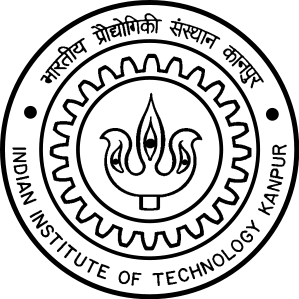
\includegraphics[width=0.25\textwidth]{./Data/iitk}
\end{center}

\vspace{3mm}
{\bf {\large {\sc DEPARTMENT OF COMPUTER SCIENCE AND ENGINEERING}}}\\
\vspace{2mm}
{\bf {\large {\sc INDIAN INSTITUTE OF TECHNOLOGY KANPUR}}}\\
\vspace{3mm}
{\textbf{ March, 2013}}\\
\end{center}
\end{singlespace}
	
\newpage
\pagenumbering{roman}
\addcontentsline{toc}{chapter}{Certificate}

\vspace {1.0in}
\begin{center}
\begin{large}
{\bf CERTIFICATE}
\end{large}
\end{center}
\vskip 0.2in
It is certified that the work contained in this 
thesis entitled ``{\bf{\textit{K-means Clustering Algorithm: Efficient Implementation on Graphics Processing Units}}}'', by {\textbf{Mr. Kunjan Aggarwal (Roll No. 10111021)}}, 
has been carried out under my supervision and this work has not been submitted elsewhere for a degree.
\vskip 1in
\begin{flushleft}
    {\bf Dr. Mainak Chaudhuri,} \\ 
    Associate Professor,\\
    Department of Computer Sc. \& Engg., \\
    Indian Institute of Technology, Kanpur\\
    Kanpur, 208016.
\end{flushleft}
	
\newpage
\addcontentsline{toc}{chapter}{Acknowledgments}

\begin{center}
\begin{large}
{\it{\bf ACKNOWLEDGMENTS} }
\end{large}
\end{center} 
\ \\ \ \\
I am greatly indebted to my supervisor Prof. Mainak Chaudhuri for his encouragement, patience and expert advice throughout the course of my study at IIT Kanpur. In spite of his busy schedule, he has always been there to help me and provide me his invaluable technical guidance and moral support. He always gave me the right direction to focus on. 

Special thanks to all my classmates of the MTech'10 batch of the Dept. of Computer Science and Engineering at IIT Kanpur for their constructive criticism of my work and for helping me out with various issues during the study. 
I especially thank Ajith Sankar for offering intuitive ideas and brain storming sessions.

My family is my source of inspiration and this thesis would have been incomplete without their support. It is my father Mr Vijay Kumar Aggarwal and my mother Mrs Sunita Aggarwal's endurance and patience that kept me motivated at all times. I could not have been successful without the never ending support from my brother Abhishek Aggarwal and my sister Sugandha Aggarwal. Finally, I would once again like to thank all my friends for insightful discussions, suggestions and encouragement. 

\ \\ \ \\
\ \\ \ \\
\vskip 0.5in
\begin{flushright}
Kunjan Aggarwal\\
March, 2013
\end{flushright}

\newpage
\addcontentsline{toc}{chapter}{Abstract}

\vspace {1.0in}
\begin{center}
\begin{large}
{\bf ABSTRACT}
\end{large}
\end{center}
\vskip 0.2in

Data analysis and classification play a big role in understanding various real life phenomena.
Clustering helps analyze data with little or no prior knowledge about it.
K-means clustering is a popular clustering algorithm with applications to computer vision, data mining, data visualization, etc.. 
Due to continuously increasing data volume, parallel computing is necessary to overcome the computational challenges involved in K-means clustering. 
We present the design and implementation of K-means clustering algorithm on widely available graphics processing units (GPUs), which have the required hardware architecture to meet these parallelism needs.
We analyze the scalability of our proposed methods with increase in number and dimensionality of data points as well as the number of clusters.
We also compare our results with current best available implementations on GPUs and a 24-way threaded parallel CPU implementation.
We achieved a consistent speedup of 6.5x over the parallel CPU implementation.

\newpage
\addcontentsline{toc}{chapter}{Contents}
\tableofcontents
\newpage
\addcontentsline{toc}{chapter}{List of Figures}
\listoffigures
\newpage
\addcontentsline{toc}{chapter}{List of Tables}
\listoftables

\newpage
\pagenumbering{arabic}
\fancyhead[RO]{\thepage}
\fancyhead[LO]{\slshape \leftmark}
\fancyfoot[CO]{}
\renewcommand{\headrulewidth}{0.5pt}
\noindent
\chapter{Introduction}
\section{Introduction}

\emph{ ``Understanding our world requires conceptualizing the similarities and differences between the entities that compose it'' } \cite{tryon}.
For understanding phenomena in real life there is always a need to aggregate all the raw data and then perform analysis over it. Various methodologies have been adopted for analyzing the raw data both for performing supervised and unsupervised learning. Clustering is one such technique, an unsupervised classification or exploratory data analysis without availability of any labeled data \cite{Xu:2009}. It aids in organizing the data instances into an efficient representation that characterizes the data being sampled.

Formally, clustering groups data instances into subsets in such a manner that similar instances are grouped together, while different instances belong to different groups \cite{lior}. The goal of clustering is to separate a finite, unlabeled data set into a finite and discrete set of ``natural'', hidden data structures, rather than to provide an accurate characterization of unobserved samples generated from the same probability distribution \cite{baraldi,mulier}.

There are a large number of clustering algorithms and heuristics that have been developed over the last many decades \cite{Jain:1999,lior,Xu:2009}. Since these clustering algorithms have to analyze real world data, they often have to deal with huge datasets that require high processing power. Over the last few years, Graphics Processing Units (GPUs) have emerged as a new alternative for handling operations with high levels of parallelism \cite{kirk}. Also since the data operations in clustering algorithms are largely independent and compute-intensive, the large number of cores available on GPUs offer a more natural alternative for extracting maximum parallelism and efficiency \cite{che_et_al}.

In our work, we will be looking at design and implementation of K-means clustering algorithm on GPUs using a general-purpose parallel programming model, namely Compute Unified Device Architecture (CUDA) \cite{cuda}. We analyze the scalability of our proposed methods with increase in number and dimensionality of data points as well as the number of clusters. We also compare our results with current best available implementations on GPUs and 24-way threaded parallel CPU implementations.

\section{Related work}

The K-means algorithm was independently proposed by Hugo Steinhaus in 1956 \cite{hugo}, Stuart Lloyd in 1957 \cite{lloyd}, Ball \& Hall in 1965 \cite{ball_hall} and James MacQueen in 1967 \cite{macqueen}.
Because of its efficiency in clustering large data sets it is one of the most popular and commonly used partitional algorithm \cite{jain:2009}.
It has been successfully used for analysis in variety of different fields like economics (market segmentation), life and medical sciences (genetics, microbiology), engineering (machine learning), astronomy, earth sciences and sociology (behavior pattern discovery) \cite{Xu:2009}. 

Initial implementations of K-means clustering algorithm on GPUs have been reported by Takizwa et al \cite{takizawa} and Cao et al \cite{cao} in 2006. Ma et al \cite{ma} made a generic translation system to port CPU code over GPUs and were able to get 20x speedup over original sequential CPU implementation. In 2007, a team at University of Virgina implemented K-means on G80 GPU and reported 8x speedup in comparison to a single threaded Pentium 4 processor \cite{che2007}. Later in 2008, they revised their work and were able to achieve 35x speedup on GTX 260 GPU over a dual core CPU \cite{che_et_al}. In 2008, another team at Hong Kong University of Science and Technology introduced GPUMiner suite \cite{gpuminer}, which contained parallel data mining implementations on graphics processors. They reported 5x improvement over the first work \cite{che2007} done by University of Virgina but it was still slower than their later implementation \cite{che_et_al}.

In 2009, a team of researchers at HP labs further improved these results \cite{wu_hp}. They achieved upto 4x speedup over university of Virgina's implementation \cite{che_et_al} and 20x to 70x speedup over GPUMiner \cite{gpuminer}. This work was further improved by Li et al \cite{li_et_al} in 2010 by making separate K-means implementations for low dimensional and higher dimensional input data sets. In 2011, Wasif et al \cite{wasif_et_al} reported 2x improvement over work of Li et al \cite{li_et_al}. They have also reported 70x speedup on Fermi architecture based GTX480 GPU over a 32 bit Intel Core 2 duo processor.

\section{Outline}
The rest of the thesis is organized as follows: In Chapter 2, we give an introduction to K-means clustering algorithm. We illustrate its different stages and then analyze its complexity and scalability. Also, we take a look into NU-MineBench benchmark suite \cite{numine} which we have used for our CPU implementations. Chapter 3 gives an overview of GPU architecture of NVIDIA's Tesla and Fermi graphics processing units. It also provides a short introduction to Compute Unified Device Architecture (CUDA) API which we have used to implement K-means on NVIDIA GPUs. Chapters 4 and 5 present details of our implementation of K-means algorithm. In Chapter 6 we show comparison of our approach with the current published results. Also, we present comparison of our results on NVIDIA GPUs with 24-way threaded parallel CPU implementations for real world datasets. Finally, Chapter 7 concludes our work and presents scope for future research.
\chapter{K-means Clustering Algorithm}
\section{Background}
Even though K-means was first proposed over fifty years ago, it is still one of the most widely used algorithms for clustering. Ease of implementation, simplicity, efficiency, and empirical success are the main reasons for its popularity.
The main features of the conventional K-means clustering algorithm \cite{hartigan} are as follows.
\begin{enumerate}
\item It is a partitional or non-hierarchical clustering method.
\item The total number of clusters, k, is assumed to be fixed and known before hand.
\item It uses Euclidean distance as the criterion for finding distance between the data points and hence, is only applicable to numerical data.
\item It is a greedy iterative method and the iterations continue till the error function has not reached a threshold or the membership of the data points no longer changes.
\end{enumerate}

\section{Algorithm}\label{sec:names}

Let $D = \lbrace x_{i}, i = 1,...,n \rbrace$ be the given input data set of $d$ dimensional data points. Let $K$ be the total number of disjoint clusters, denoted by $C = \lbrace c_{k}, k = 1,...,K\rbrace$. For each cluster $c_{k}$ let $\mu\left( c_{k}\right) $ be its centroid or mean. Then the error function is defined as $$E\left( C\right) = \sum_{k=1}^{K}{\sum_{x\epsilon c_{k}}^{}{\Vert x - \mu\left( c_{k}\right)\Vert^{2} }}$$
The aim of K-means is to minimize the value of the error function $E\left(C)\right)$ which is an NP-hard problem \cite{drineas}.

The pseudo code for conventional K-means algorithm is shown in Algorithm \ref{algo:kmean}. 
\begin{algorithm} 
\caption{\textsc{K-means Algorithm}}
\label{algo:kmean}
\begin{algorithmic}[1]
\REQUIRE Dataset $D$ containing $n$ $d$-dimensional points, Number of clusters $K$, Error threshold $E_{t}$
\ENSURE $K$ disjoint clusters, $C = \lbrace c_{k}, k = 1,...,K\rbrace$ with their members.
%\STATE Initialization()
\STATE $\lbrace c_{1},c_{2},...,c_{k}\rbrace$ be the initial $K$ partitions.\label{algo:kmean:init}
\REPEAT
%\STATE FindNearest()
\FORALL{data-point $x$ in $D$} \label{algo:kmean:nearest}
	\STATE Let $x$ belongs to cluster $c_{1}$.
	\STATE $min_{dist} \gets \Vert x - \mu \left(c_{1}\right)\Vert^{2}$
	\FORALL{centroid $\mu$}
		\STATE $dist \gets \Vert x - \mu\Vert^{2}$
		\STATE If $dist < min_{dist}$, assign $x$ to $\mu$
	\ENDFOR
\ENDFOR
%\STATE Compute()
\STATE Recompute the cluster centroids based on above assignments. \label{algo:kmean:compute}
\STATE Calculate the error function $E\left(C\right)$.
\UNTIL either there were no changes in cluster membership or value of $E\left(C\right) < E_{t}$. \label{algo:kmean:term}
\end{algorithmic}
\end{algorithm}


\section{Analysis}
K-means algorithm tries to terminate at a local optimum. It always converges to a local minimum point \cite{selim} after a finite number of iterations and so the value of error function $E\left(C\right)$ is always non-increasing.
The most important choice for K-means algorithm is the choice of value $K$. Also, the final set of clusters and the number of iterations taken to reach them is dependent on the initially selected centroids (Step \ref{algo:kmean:init} in Algorithm \ref{algo:kmean}). Figure \ref{fig:kmean} illustrates the execution of K-means Algorithm \ref{algo:kmean}.

\begin{figure}[h]
	\centerline{
   \subfloat[Initial Phase]{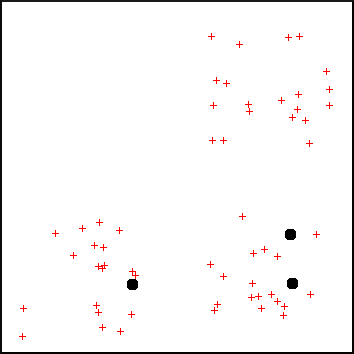
\includegraphics[width=0.3\textwidth]{./Data/kmeans_algo/initial}  	\label{fig:kmean_init} }
   \subfloat[$1^{st}$ Assignment]{	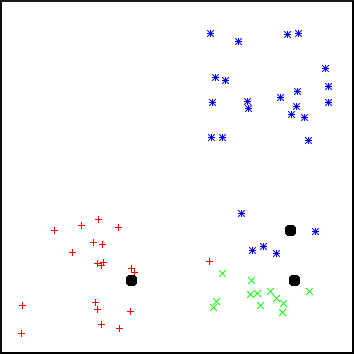
\includegraphics[width=0.3\textwidth]{./Data/kmeans_algo/first_assign}  	\label{fig:kmean_assign1} }
   \subfloat[$1^{st}$ Re-computation]{	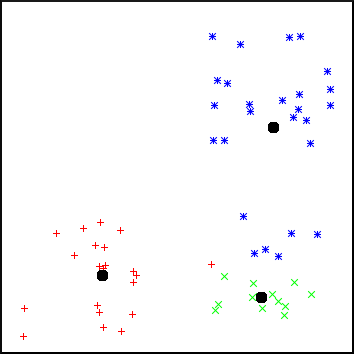
\includegraphics[width=0.3\textwidth]{./Data/kmeans_algo/first_compute}  	\label{fig:kmean_compute1} }
   }

	\centerline{
   \subfloat[$2^{nd}$ Assignment]{	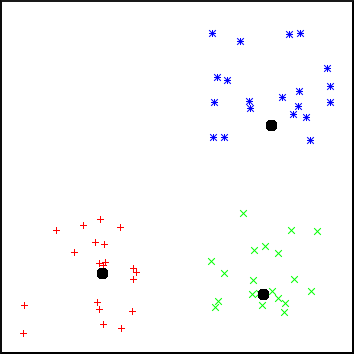
\includegraphics[width=0.3\textwidth]{./Data/kmeans_algo/second_assign}  	\label{fig:kmean_assign2} }
   \subfloat[$2^{nd}$ Re-computation]{	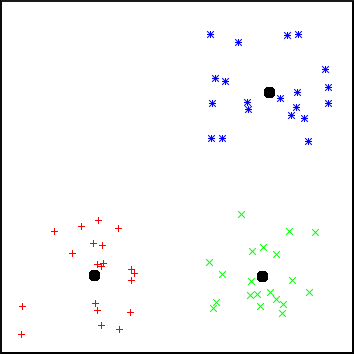
\includegraphics[width=0.3\textwidth]{./Data/kmeans_algo/second_compute}  	\label{fig:kmean_compute2} }
   \subfloat[Final Assignment]{	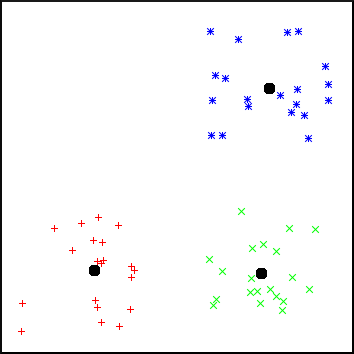
\includegraphics[width=0.3\textwidth]{./Data/kmeans_algo/third_assign}  	\label{fig:kmean_assign3} }
	}
	\caption{Illustration of the K-means Algorithm \ref{algo:kmean} for two-dimensional data points when number of clusters, $K = 3$}
\label{fig:kmean}
\end{figure}

We consider the case where the input data points are two-dimensional and the value of $K$ is 3. Figure \ref{fig:kmean_init} shows the initialization phase (Step \ref{algo:kmean:init}) of the algorithm. Three random data-points have been selected as the initial centroids. In the first iteration, the assignment stage (Step \ref{algo:kmean:nearest}) assigns the data points to the initial centroids based on their Euclidean distance with the initially selected centroids as depicted in Figure \ref{fig:kmean_assign1}. In the re-computation stage, (Step \ref{algo:kmean:compute}) the centroids are re-computed to their new values (Figure \ref{fig:kmean_compute1}).

In the second iteration, during assignment of data points many points change their cluster (Figure \ref{fig:kmean_assign2}). Due to this re-assignment there is again a shift in the positions of the centroids (Figure \ref{fig:kmean_compute2}). As we can visually see, the centroids are moving closer to the actual cluster centers with each iteration. This gives a general idea of how the algorithm converges to the final clusters and why the value of error function $E\left(C\right)$ keeps on decreasing with each iteration \cite{selim}.

Finally, in the third and last iteration assignment stage does not produce any reassignments (Figure \ref{fig:kmean_assign3}). Since this was our termination condition (Step \ref{algo:kmean:term}), the algorithm exits and outputs the final clusters with their members.

\subsection{Finding nearest centroids}\label{sec:findnearest}
During assignment of the $n$ data points, distance of each data point is calculated from all the $K$ clusters. Assuming input data to be $d$-dimensional, this takes $O(nKd)$ time. Finding the minimum distance out of the $K$ distances for all $n$ data points takes $O(nK)$ time. Thus, the total time complexity of this step is $O(nKd + nK)$. For large input data sets, values of $d$ and $K$ are much smaller as compared to $n$. As a result, we can consider this step to be linear in terms of $n$. 

Also, the extra space required is for storing the membership of the data points which anyways is required in the output and is again $O(n)$. Hence, the time and space complexity have a linear increase with increase in the size of input data set, making it highly scalable.

\subsection{Computing new centroids}
While computing new centroids, value $\mu$ is calculated for each of the $K$ clusters. This requires taking mean of all the members for every cluster. Since these clusters are disjoint, mean calculation of all the $K$ clusters has a time complexity of $O(nd)$. Again for large data sets this can be considered linear in terms of $n$.

For storing the computed $K$ centroids it requires $O(Kd)$ extra space. Hence, this step too is linear in terms of $n$ making the complete K-means algorithm linear and very efficient for large sized data sets.

\section{NU-MineBench: A CPU Benchmark}
In this section we will take a look at NU-MineBench data mining benchmark suite \cite{numine} developed at Northwestern University. This suite contains parallel implementations of various data mining algorithms, including K-means, on CPU. Previous authors \cite{gpuminer, che_et_al, wu_hp} have used NU-MineBench for their CPU implementation of K-means while comparing runtime of their GPU implementations with CPU. That's why, we too decided to use the same to benchmark our work on GPU against CPU. 

\subsection{Implementation Details}
NU-MineBench uses OpenMP API \cite{openmp} to execute K-means in parallel across maximum possible threads available on CPU. The CPU-based implementation is illustrated in Algorithm \ref{algo:numine}.

\begin{algorithm} 
\caption{\textsc{K-means Algorithm from NU-MineBench}}
\label{algo:numine}
\begin{algorithmic}[1]
\REQUIRE Dataset $data[n][d]$, Number of clusters $K$, Maximum iterations $M_{itr}$
\ENSURE $centroid[K][d]$, $membership[n]$.
%\STATE Initialization()
\FORALL{cluster $k$ in $K$} \label{algo:numine:init}
	\FORALL{dimension $d_{i}$ in $d$}
		\STATE $centroid[k][d_{i}] \gets data[k][d_{i}]$
	\ENDFOR
\ENDFOR
\STATE Let $T$ be maximum number of threads.
\REPEAT
%\STATE FindNearest()
\STATE Partition the $n$ data points equally among all $T$ threads. \label{algo:numine:nearest}
\STATE Initialize all values in $newClusterSize[T][K]$ to $0$.
\STATE Initialize all values in $newCentroid[T][K][d]$ to $0$.
\STATE Start parallel execution for each thread $t$ in $T$.
\FORALL{data-point $p$}
	\STATE Compute nearest centroid $k$ amongst $centroid[K][d]$.
	\STATE $membership[p] \gets k$
	\STATE $newClusterSize[t][k]{+}{+}$
	\FORALL{dimension $d_{i}$ in $d$}
		\STATE $newCentroid[t][k][d_{i}]\ {+}{=}\ data[p][d_{i}]$
	\ENDFOR
\ENDFOR	
\STATE End parallel execution.
%\STATE Compute()
\FORALL{cluster $k$ in $K$} \label{algo:numine:compute}
	\FORALL{thread $t$ in $T$}
		\STATE $newClusterSize[0][k]\ {+}{=}\ newClusterSize[t][k]$
		\FORALL{dimension $d_{i}$ in $d$}
			\STATE $newCentroid[0][k][d_{i}]\ {+}{=}\ newCentroid[t][k][d_{i}]$
			\STATE $centroid[k][d_{i}] \gets newCentroid[0][k][d_{i}] / newClusterSize[0][k]$
		\ENDFOR
	\ENDFOR
\ENDFOR
\UNTIL either there were no changes in $membership[]$ or maximum iterations $M_{itr}$ have been completed. \label{algo:numine:term}
\end{algorithmic}
\end{algorithm}


Since, it is hard to know the number of iterations it might take for the K-means to end, NU-MineBench takes the maximum number of iterations $M_{itr}$ as an additional input. Step \ref{algo:numine:init} initializes the first $K$ data points as the initial centroids. During assignment of data points (Step \ref{algo:numine:nearest}) to their nearest centroids, maximum possible threads are launched on CPU. The data points are equally partitioned among all the threads. For independent parallel execution, each thread maintains its own cluster variables, $newClusterSize$ containing the number of points that are member of each cluster and $newCentroid$ storing the sums of dimensions of all the assigned data points for every cluster. For every data point, index of its nearest cluster is stored in $membership$ variable and the $newClusterSize$ and $newCentroid$ variables of that centroid are updated.
 
After all the threads have finished evaluating their data points and stored values in their respective $newClusterSize$ and $newCentroid$ variables, the parallel execution ends. Now a single thread (main thread) reduces these values obtained by each thread for every cluster (Step \ref{algo:numine:compute}). In the end, the new centroids are computed by taking mean of all the data points that had been assigned to each cluster and are assigned to $centroid[]$.

At the end of an iteration, if there was no change in $membership[]$ or if we have finished $M_{itr}$ iterations than $centroid[]$ and $membership[]$ are returned as the final results of K-means.

\subsection{Our Modifications}\label{sec:cpuMod}
NU-MineBench's performance relies heavily on cache utilization. To avoid any shared memory conflicts between the parallel executing threads, local variables $newClusterSize$ and $newCentroid$ are maintained separately for each thread. Also, while computing new centroids (Step \ref{algo:numine:compute}) only a single thread is used because the overhead of launching multiple threads to perform a tree-based reduction is much higher than doing flat reduction using a single thread. This is based on the assumption that the total number of available threads are going to be low keeping the number of values to be reduced small.

But we found that speedup achieved with NU-MineBench decreases as the value of $K$ is lowered. In fact, for $K = 2$, we saw an increase in execution time with increase in thread count; see Figure \ref{fig:numine:orig}. On investigation we found false sharing to be the limiting factor. While assigning memory for variable $newClusterSize$, a continuous memory space of size $T*K*sizeof(int)$ bytes is allocated in memory, where first $K$ positions are updated by first thread, next $K$ by second thread and so on. When the value of $K$ is small it is possible that values for multiple threads reside in the same cache block. This results in multiple threads updating the same cache block and so the participant threads have to update the values in their cache with changes done by other threads before doing a read.

\begin{figure}[h]
	\centerline{
   \subfloat[Original NU-MineBench]{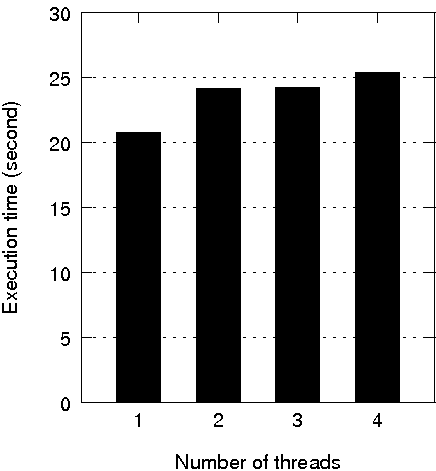
\includegraphics[width=0.4\textwidth]{./Data/numine/original}  	\label{fig:numine:orig} }
   \subfloat[Modified NU-MineBench]{	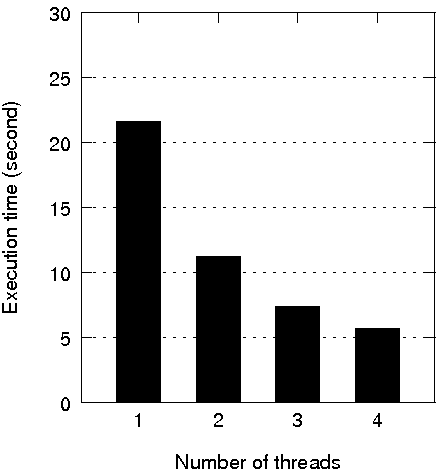
\includegraphics[width=0.4\textwidth]{./Data/numine/modified}  	\label{fig:numine:mod} }
	}
	\caption{Execution times of NU-MineBench based K-means Algorithm \ref{algo:numine} for 100 iterations on Record Linkage Dataset \cite{recordLinkage}, with $K = 2$, $d = 9$, $n = 5749132$. (a) Original NU-MineBench shows slight increase in execution time with increase in thread count due to latencies caused by false sharing. (b) Modified NU-MineBench shows linear speedup with increase in thread count.}
\label{fig:kmean}
\end{figure}


To overcome this shortcoming we ensure that the values stored by each thread occupy distinct cache blocks. We separate every set of $K$ indices inside the array $newClusterSize$ with unused memory locations. We also make similar changes for $newCentroid$ array. This ensures that even for smaller values of $K$ the speedup obtained is linear in thread count; see Figure \ref{fig:numine:mod}. Also, since the size of the cache block is generally small (typically 64 bytes), this change does not make any significant impact on the overall memory requirement.

\chapter{CUDA: A General Purpose Parallel Computing Architecture}
The first ever commercial graphics processing unit (GPU) was designed by NVIDIA in 1999. Because of the ever increasing demand for producing real-time graphics, which requires high arithmetic throughput, manufacturers have always focused on increasing the parallel processing capabilities of the GPUs. Today, GPUs outperform CPUs both in arithmetic processing efficiency and memory bandwidth \cite{nickolls,glaskowsky}.

Since 2003, efforts have been made to use GPUs even for non-graphics applications, especially for scientific work so that their high arithmetic throughput can be fully exploited. In our work we have used NVIDIA's Tesla C1060 and Fermi-based Tesla C2070 GPU cards. For implementing K-means algorithm on GPU, we have used Compute Unified Device Architecture (CUDA) \cite{cuda} API. This chapter will provide a brief introduction to NVIDIA's GPU architecture and CUDA API. More detailed information is available in literature published by NVIDIA \cite{cudadocs,fermiWhitepaper} and in books written by Farber \cite{farber} and Kirk \cite{kirk}.

\section{GPU Architecture}
\subsection{Overview}
Tesla C2070 is based on NVIDIA's Fermi architecture. It contains 448 CUDA cores. These cores are organized in 14 Streaming Multiprocessors (SMs) each containing 32 cores or Streaming Processors(SP). Figure \ref{fig:fermi:arch} shows block diagram of Fermi GF100 GPU containing 16 SMs, two more than C2070 GPU card that we have used for our work. Figure \ref{fig:fermi:arch} also shows six 64-bit DRAM memory partitions that provide a 384-bit memory interface. C2070 can support 6GB of GDDR5 DRAM memory. For data transfer between CPU and GPU there is a host interface connecting GPU with CPU via PCI-Express.

\begin{figure}[h]
	\centerline{
   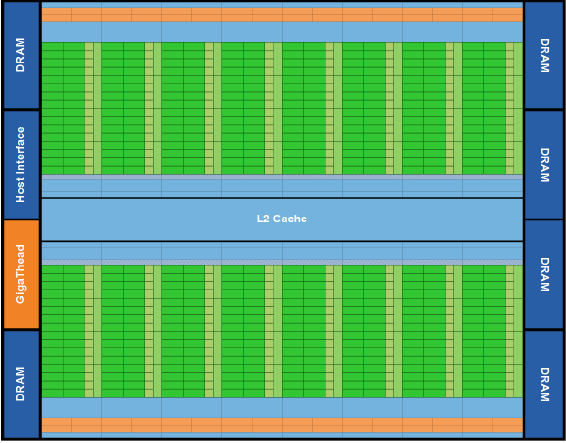
\includegraphics[width=0.8\textwidth]{./Data/nvidia/architecture_fermi}  	
	}
	\caption{ Block Diagram of G100 Fermi GPU containing 16 Streaming Multiprocessors (SMs) (Source: NVIDIA \cite{fermiWhitepaper}).}
\label{fig:fermi:arch}
\end{figure}

Fermi uses a {\it GigaThread} global scheduler to distribute execution blocks between the SMs. Each SM contains unified graphics and computing multiprocessors which execute vertex/geometry shader programs as well as parallel computing programs. We will be concentrating only on the parallel computing capabilities of SMs. A typical Fermi SM is shown in figure \ref{fig:fermi:sm}. Each SM contains 32 SIMT (Single-Instruction, Multiple-Thread) cores. 

\begin{figure}[h]
	\centerline{
   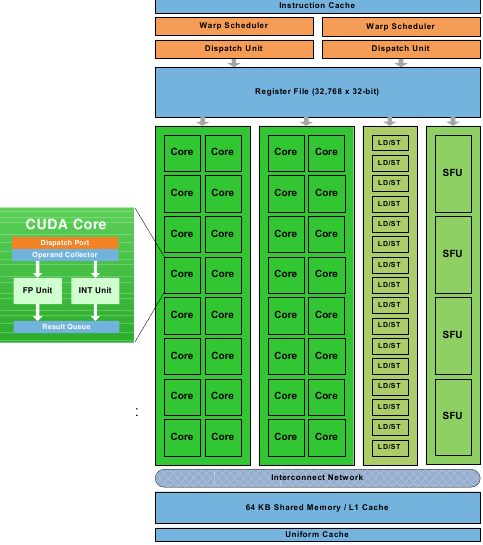
\includegraphics[width=0.8\textwidth]{./Data/nvidia/sm_fermi}  	
	}
	\caption{ Block Diagram of Fermi Streaming Multiprocessor (SM) containing 32 cores (Source: NVIDIA \cite{fermiWhitepaper}).}
\label{fig:fermi:sm}
\end{figure}

Each core contains a fully pipelined integer arithmetic logic unit (ALU) and floating point unit (FPU). Also, there are sixteen load/store units (LD/ST) to calculate source and destination addresses for sixteen threads per clock. Each SM contains four Special Function Units (SFUs) which execute transcendental instructions like sine, cosine and square root. Apart from register file, used for storing private variables, each SM also contains on-chip memory that is used for caching and sharing data between the cores. The instructions are fetched from instruction cache and are dispatched to the cores by two warp schedulers. More details about the on-chip memory and the warp schedulers is provided in the later sections.

\subsection{Memory Hierarchy}

Data reuse is an essential requirement for GPUs. This is due to the high latency of DRAM memory. To overcome this challenge caches have been provided, both inside SMs and also between the SMs and global memory, to cache regularly accessed data. Figure \ref{fig:fermi:mem} shows various memory partitions present in Fermi.

\begin{figure}[h]
	\centerline{
   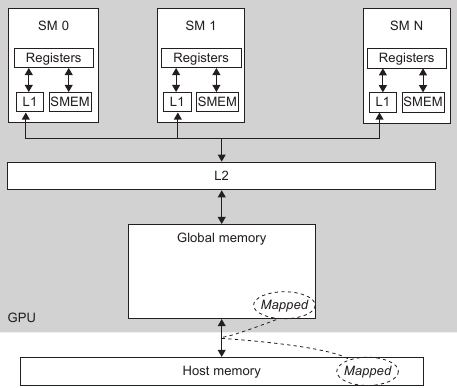
\includegraphics[width=0.8\textwidth]{./Data/nvidia/mem_fermi}  	
	}
	\caption{ CUDA memory hierarchy. (Source: NVIDIA \cite{farber}).}
\label{fig:fermi:mem}
\end{figure}

The global memory is stored in an external DRAM. It is used for communication between the SMs. Also any data transferred between CPU and GPU is also stored here. It is essential to coalesce global memory accesses to ensure single wide memory transactions. All the data accesses (both reads and writes) get cached in the unified L2 cache in an LRU fashion. It is 768 KB in size and helps in speeding up irregular accesses from global memory. Also it is coherent, ensuring all the cores receive updated values.

To further optimize data access from global memory a separate on-chip L1 cache is also present on each SM. It only caches memory reads and any stores directly go to L2 cache. It has been provided for exploiting spatial locality and uses 128  byte wide transactions. To make the L1 cache more configurable, it can be divided into L1 cache (maintained by SM) and shared memory (programmable). Shared memory can occupy either 16 KB or 48 KB from the 64 KB L1 cache. By storing data inside shared memory, the programmer can ensure that data which has to be reused over a long period of time stays inside the on-chip cache. L1 cache is shared between all the executing cores but unlike L2, it is not coherent and requires careful measures to ensure coherence.

Each executing core maintains its private data inside 32 K 32-bit registers. During execution the registers get partitioned among the cores statically and this partitioning can not be reconfigured till the execution finishes. As a result, if the private data cannot fit inside the available registers, it is spilled into the local memory. Fermi tries to accommodate the spilled data inside L1 cache which may lead to eviction of cached data.

Constant memory and texture memory are two other memory types present in Fermi. They both get cached on-chip and were of high importance in earlier models of NVIDIA GPUs because of unavailability of L2 and L1 caches. Constant memory is 64 KB in size and is read-only. In fact, one can get the same performance as from constant memory by declaring the data as constant inside global memory. Still, constant memory might become important if L2 cache is unable to accommodate all the data. But constant memory has a strong limitation. It only allows access of a single memory location at one time. Texture memory used to give better performance in comparison to global memory for non-coalesced data access on older GPUs. But with availability of L2 and L1 cache on Fermi, its advantage over global memory is very limited. It is more useful for visualization and shader programming.

\subsection{Hardware Multithreading}
A thread is the smallest execution unit on a GPU. Threads are created, managed, scheduled and executed by SM's SIMT multithreaded instruction unit in groups of 32 parallel threads called warps. Fermi SMs contain two warp schedulers which independently schedule alternate warps (see Figure \ref{fig:fermi:warp}). While one warp scheduler handles all the even warps, the other handles all the odd warps.
\begin{figure}[h]
	\centerline{
   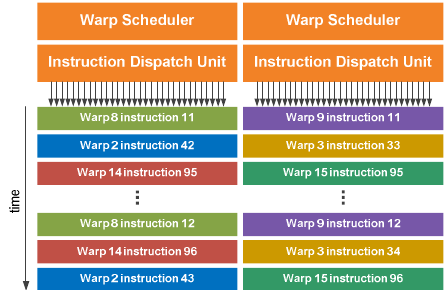
\includegraphics[width=0.8\textwidth]{./Data/nvidia/warp_fermi}  	
	}
	\caption{ Single-Instruction, Multiple-Thread (SIMT) warp execution on Fermi.(Source: NVIDIA \cite{fermiWhitepaper}).}
\label{fig:fermi:warp}
\end{figure}


A SIMT warp is composed of individual threads of the same type. All the threads start together at the same program address. Whenever the cores assigned to a warp scheduler are ready, the scheduler selects a warp that is ready to execute and issues the next instruction on that warp's active threads. The instruction gets broadcast to all the participant threads.

Due to branching and predication, a thread may be inactive and may not execute. Whenever threads diverge, all the branches are executed serially. All the threads that do not fall on a particular path are disabled. Once all the paths have been completed the participant threads again re-converge and start executing the next instruction simultaneously.

Serial execution due to branch divergence only happens inside a warp. Different warps can independently execute common or disjoint paths without effecting each other. Since each warp scheduler has 16 cores to execute upon, an issued warp instruction executes as two sets of 16 threads (half-warps) over two processor cycles. Also, the maximum number of warps that can reside simultaneously on an SM gets decided by the availability of resources (registers and shared memory).

\section{CUDA API}
\subsection{CUDA Execution Model}
During execution of CUDA programs, the program is executed with the GPU acting as a co-processor of CPU. While executing a GPU program, the code starts execution on the CPU. To ask the CPU to execute a piece of code on the GPU, a special call called kernel invocation is used. It is an asynchronous call to the CUDA driver which loads the program on GPU and control immediately comes back to the CPU to execute the next instruction. 
\begin{figure}[h]
	\centerline{
   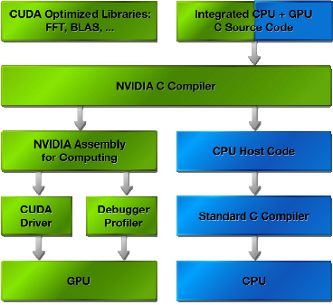
\includegraphics[width=0.6\textwidth]{./Data/nvidia/cuda_fermi}  	
	}
	\caption{ CUDA software stack.(Source: NVIDIA).}
\label{fig:fermi:cuda}
\end{figure}

All transfers of data, launching of GPU computing functions (kernels) and any other interaction between CPU and GPU are handled by the runtime driver. To map a large computational problem on the highly parallel GPU architecture, the problem is divided into smaller independent components that can be solved in parallel.

Before scheduling the large number of concurrent threads on to the GPU, they are partitioned into disjoint components called thread blocks. All threads in a thread block co-operate with each other and run on a single SM, executing the same set of instructions. Since the threads inside a block are present on the same SM, they can share the data among each other through shared memory and with constituent threads of other blocks through global memory.

While threads in a single warp always execute in a synchronized manner, the threads in a thread block can also synchronize using barrier synchronization functions. During kernel invocation, the total number of thread blocks and the number of threads present in each block need to be specified. On the basis of this information the resource usage (shared and register memory) of each block is calculated. The {\it GigaThread} scheduler then allocates maximum possible blocks to each SM.

After receiving the thread blocks, SM divides them into warps and allocates them to the warp schedulers. Finally, the two warp schedulers pick up one warp each which is ready to execute and start executing instructions. The remaining blocks which could not be allocated any SM wait for the current set of blocks to finish their execution. New thread blocks are only allocated to an SM after it has finished execution of all the thread blocks currently allotted to it.

\subsection{CUDA C Runtime}
For programming using CUDA, we have used CUDA's C Runtime API. We mention here few basic functions provided by the C runtime. An exhaustive listing is present in CUDA reference manual \cite{cuda}.
\begin{itemize}
\item {\bf Kernel invocation:} A kernel is declared like a normal C function except that it uses the qualifier, \_\_global\_\_.


\begin{lstlisting}
__global__ void firstKernel (void) {
}
\end{lstlisting}


While invoking a kernel we need to pass two parameters to it which specify the way thread blocks and threads inside individual thread blocks are going to be organized.

\begin{lstlisting}
firstKernel << grid_size, block_size >> ();
\end{lstlisting}

Here {\it grid\_size} specifies the grid size for blocks and {\it block\_size} specifies the grid size for threads inside every block.

\begin{lstlisting}
dim3 grid_size (gx, gy, gz);
dim3 block_size (bx, by, bz);
\end{lstlisting}

During kernel execution, each block and every thread inside it is assigned an index on the basis of their position in the grids we defined above.

\item {\bf Device functions:} Device functions use the qualifier \_\_device\_\_. A device function can only be invoked from code running on GPU.

\begin{lstlisting}
__device__ void firstDevice ( void ) {
}
__global__ void firstKernel ( void ) {
  firstDevice();
}
\end{lstlisting}

Also, Fermi GPUs allow device functions that are recursive in nature.


\item {\bf Memory allocation:} To allocate variables in device memory we use the function, {\it cudaMalloc}.

\begin{lstlisting}[morekeywords={cudaMalloc,cudaMemcpy,cudaMemcpyHostToDevice}]
// Allocate array in host memory
float *h_A = (float *)malloc(size);
// Allocate array in device memory
float *d_A;
cudaMalloc ( &d_A, size );
// Copy array from host memory to device memory
cudaMemcpy ( d_A, h_A, size, cudaMemcpyHostToDevice );
\end{lstlisting}

{\it cudaMemcpy} is used to copy data from host to device memory, or from device to device memory and from device to host memory.

\item {\bf CUDA events:} For performance benchmarking and runtime measurement, we have used events provided by CUDA.

\begin{lstlisting}[morekeywords={cudaEvent_t,cudaEventCreate,cudaEventRecord,cudaEventSynchronize,cudaEventElapsedTime,cudaEventDestroy}]
// Create the event variables.
cudaEvent_t start, stop;
cudaEventCreate(&start);
cudaEventCreate(&stop);

// Record the event when kernel starts.
cudaEventRecord(start, 0);
{
  firstKernel << grid_size,block_size >> ();
}
// Record the event when kernel stops.
cudaEventRecord(stop, 0);
// Wait for the asynchronous kernel to finish.
cudaEventSynchronize(stop);
// Store the elapsed time.
float elapsedTime;
cudaEventElapsedTime ( &elapsedTime, start, stop );

// Finally destroy the event variables.
cudaEventDestroy(start);
cudaEventDestroy(stop);
\end{lstlisting}
\end{itemize}


\chapter{Finding Nearest Centroid}
In this chapter we will create a parallel implementation for assigning  data points to their nearest cluster. As explained in Section \ref{sec:findnearest}, the time complexity of this step is linear in terms of the number of data points. Also, calculation of distance for each data point does not depend on any other data point and so processing for all the data points can continue in parallel.

We will pay special attention to the arrangement of data points and centroids inside GPU memory. Also, because of the limited on-chip memory available in a GPU core we need to optimize our implementation such that loading of data points inside on-chip memory is in parallel with distance calculation, so that the cores are never idle.

We will start with an implementation for the special case where the input data points are low-dimensional. We will look at the various possible storage arrangements and their effect on the processing efficiency. On the basis of our observations for the special case of low-dimensional data points, we will finally create a generic implementation which can efficiently parallelize assignment of data points of any dimension and is fully scalable.

We will continue to use the naming convention introduced in Section \ref{sec:findnearest}. For all remaining chapters same naming convention will be used.

\section{Special Case: Low-dimensional Input}
We will consider the case where the dimension $d$ of input data is small enough to load one complete data point inside the on-chip registers available to a thread. Since, the number of registers available per thread are limited (64 and 128 in C2070 and C1060 respectively), we will only be considering inputs with value of $d$ up to 22.

Each thread will be assigned a data point. It will calculate the distance of the data-point from all the $k$ centroids. The index of the nearest centroid will be stored in an array of length $n$ and will be the final output.
\subsection{Storage of data points}\label{sec:dataStorage}
The data points are stored in device memory as it has the maximum capacity. Also, once copied into the device memory the data points will never need to be re-arranged so the cost of copying data from host memory to device memory is one time.

While loading the data points from device memory, threads belonging to the same  warp load the same dimension of successive data points. To ensure that each load by a warp completes in a single transaction the data points are arranged as $[d][n]$ i.e. first dimension of all data points, followed by second dimension of all data points and so on.

Still, if value of $n$ is not a multiple of transaction-width of device memory, a single read by warp might require two transactions. To avoid this we use $cudaMallocPitch$ function to allocate memory for data points with padding, ensuring that first value for each dimension starts at transaction boundary. $cudaMemcpy2D$ is used to copy the data from host into this padded memory.

\subsection{Loading of data points}
Since a data-point can be completely loaded inside a thread, all the threads load their data points only once at the beginning of the kernel. While declaring the register array inside a thread we can't use a variable $d$ for specifying array length. So instead we create a kernel template with dimension $d$ as template variable. At the time of invocation of kernel, we specify the value $d$ as a constant.

\begin{lstlisting}[morekeywords={blockIndx,blockDim,threadIdx},breaklines=true]
//Create the kernel template.
template <int d>
__global__ void findNearest (int n, float *datapoint, int K, float *membership) {
	float point[d];
	// Get the index of the data point to be processed
	int index = blockIndx.x * blockDim.x + threadIdx.x;
	// Load the complete data point
	# pragma unroll 
	for (int dim=0; dim<d; dim++) {
		point[dim] = datapoint[n*dim + index];
	}
	//Calculate distance from each centroid one by one.
	for ( int k=0; k<K; k++) {
		//Get distance from current centroid
		dist = getDist(k);
		//If distance is less than minimum distance then update it.
		if (dist < min) {
			nearest = k;
			min = dist;
		}
	}
	//Store index of centroid with minimum distance.
	membership[index] = nearest;
}
// kernel template invocation.
switch (d) {
  case 1:  findNearest<1> <<grid_size, block_size>> (..);
           break;
  case 2:  findNearest<2> <<grid_size, block_size>> (..);
           break;
       .
       .
  case 22: findNearest<22> <<grid_size, block_size>> (..);
           break;
}			
\end{lstlisting}

\subsection{Loading of centroids}
All the threads need to access the same $K$ centroids. This gives an excellent opportunity for reusing the centroid values loaded from device memory. This can be done by loading the centroids in shared memory. Also, all the threads inside a warp access the same dimension of a single centroid. Due to this broadcast access, constant memory can also be used for storing the centroid. We compare both the approaches.
\subsubsection{Centroid in shared memory}
We consider the optimum case where value $K$ and $d$ are such that all the centroids can be accommodated in the shared memory at once. All the threads after loading their data points, load all the centroids in shared memory. 

Threads in the same block wait till all the threads finish loading the centroids to ensure that all centroid values have been loaded into shared memory. Once centroids are loaded no more device memory accesses are required and each thread computes the distance from all the centroids by using data point present in its on-chip registers and centroids present in shared memory. Finally, the index of the closest centroid is stored in the membership array in a coalesced manner.
\subsubsection{Centroid in constant memory}\label{sec:centConstt}
In the case of access from constant memory, once the data point has been loaded by a thread, it can directly start accessing the centroid values for distance computation. Also, since each thread first computes distance from one centroid before moving onto the next centroid, we store centroids as $[K][d]$ to ensure spatial locality inside constant memory cache.
\subsubsection{Centroid in device memory}
For the case of Fermi, data in device memory is also cached (until written to) in on-chip $L1$ cache. So for C2070, we also try accessing centroid directly from device memory instead of loading it into shared memory. In this case also, after loading of data points each thread can directly start computing the distance from centroids. We set the size of the $L1$ cache to 48KB, so that more space is available for caching the centroids.

\subsubsection{Analysis}
Tables \ref{table:lowC1060} and \ref{table:lowC2070} show the comparison of runtime on C1060 and C2070 for the different approaches discussed above. Second last column in each table shows the time taken to execute the kernel when the centroids are accessed from shared memory but the centroid values are not loaded from device memory.

On comparing the second last and third last columns we can conclude that the time taken in loading of centroids in shared memory from device memory does not have much impact on the runtime.

\begin{table}[htbp]
\begin{center}
\begin{tabular}{|p{2cm}|p{1cm}|p{1cm}|p{2.5cm}|p{2.5cm}|p{2.5cm}|}
\hline
\multicolumn{1}{|c|}{n} & \multicolumn{1}{c|}{k} & \multicolumn{1}{c|}{d} & \multicolumn{1}{p{2.5cm}|}{Centroid in shared (ms)} & \multicolumn{1}{p{2.5cm}|}{Centroid in shared (no loading) (ms)} & \multicolumn{1}{p{2.5cm}|}{Centroid in constant (ms)} \\ \hline
1000000 & 100 & 2 & 144.949 & 136.497 & 101.8 \\ \hline
1000000 & 100 & 4 & 226.485 & 214.307 & 189.069 \\ \hline
1000000 & 100 & 6 & 310.873 & 295.749 & 256.848 \\ \hline
1000000 & 100 & 8 & 395.369 & 377.717 & 324.207 \\ \hline
1000000 & 100 & 10 & 478.628 & 460.491 & 390.703 \\ \hline
1000000 & 100 & 12 & 563.822 & 542.453 & 457.283 \\ \hline
1000000 & 100 & 14 & 649.383 & 625.637 & 522.894 \\ \hline
1000000 & 100 & 16 & 733.757 & 707.335 & 588.915 \\ \hline
1000000 & 100 & 18 & 819.075 & 790.253 & 654.948 \\ \hline
1000000 & 100 & 20 & 902.335 & 872.237 & 721.292 \\ \hline
1000000 & 100 & 22 & 987.537 & 954.896 & 788.082 \\ \hline
\end{tabular}
\end{center}
\caption{Comparison of runtime for 50 iterations of label assignment on C1060 for low-dimensional data with different access locations for centroid.}
\label{table:lowC1060}
\end{table}

For C1060, constant memory gives much better performance than shared memory. It also outperforms the case when there is no loading delay in shared memory. This clearly shows that the accesses from the constant cache are much faster than those from the shared memory. Our benchmarking experiments also showed that throughput achieved from shared memory accesses is three-fourth of the throughput achievable by register accesses.

For the last row in Table \ref{table:lowC1060}, shared memory without any load latency achieves 345 GFlop/s whereas constant memory achieves 418 GFlop/s. With a single instruction executing every cycle, C1060 can achieve 311 GFlop/s for single precision floating point operations. During distance calculation, the typical operations are as follows.
\begin{lstlisting}[breaklines=true]
distance += (point[i] - centroid[i])*(point[i] - centroid[i]);
\end{lstlisting}

This can be broken down into one $ADD$ operation to calculate the difference for the $i^{th}$ dimension followed by a $MAD$ operation that squares the difference and adds it into $distance$ variable. Both $ADD$ and $MAD$ operations take one cycle each. So every distance updation takes two cycles and performs three single-precision floating point operations.

C1060 also allows us to perform a $MUL$ operation in parallel with a $MAD$ provided the operands are different. To use the parallel $MUL$ operation, the distance calculation can be modified as:
\begin{lstlisting}
temp1 = (point[i] - centroid[i]);        // ADD
temp2 = (point[i+1] - centroid[i+1]);    // ADD
distance += temp1*tmp1; temp2 *= temp2;  // MAD + MUL
distance += temp2;                       // ADD
\end{lstlisting}
Here two $distance$ updations are coupled together to use a $MUL$ operation in parallel with $MAD$ operation. But this too takes four cycles for two updations. Hence, maximum possible throughput for distance calculation is $311 * (3/2)$ i.e. 466 GFlop/s. With constant memory, we are able to achieve almost $89\%$ of this peak throughput.

On C2070, the $L1$ cache used for caching accesses from global memory is not able to perform as well as the cache provided by constant memory. Here also, when the centroids are in shared memory, loading of centroids from device memory causes very small overhead, as can be seen by comparing the second last and the third last columns of Table \ref{table:lowC2070}.


\begin{table}[htbp]
\begin{center}
\begin{tabular}{|p{1.6cm}|p{0.8cm}|p{0.5cm}|p{2.2cm}|p{2.2cm}|p{2.2cm}|p{2.2cm}|}
\hline
\multicolumn{1}{|c|}{n} & \multicolumn{1}{c|}{k} & \multicolumn{1}{c|}{d} & \multicolumn{1}{p{2.2cm}|}{Centroid in global (ms)} & \multicolumn{1}{p{2.2cm}|}{Centroid in shared (ms)} & \multicolumn{1}{p{2.2cm}|}{Centroid in shared (no loading) (ms)} & \multicolumn{1}{p{2.2cm}|}{Centroid in constant (ms)} \\ \hline
1000000 & 100 & 2 & 108.5 & 96.95 & 93.7 & 95.462 \\ \hline
1000000 & 100 & 4 & 168.3 & 145.3 & 142.9 & 142.994 \\ \hline
1000000 & 100 & 6 & 227.65 & 195.2 & 189.65 & 190.869 \\ \hline
1000000 & 100 & 8 & 286.3 & 244.55 & 239.6 & 238.95 \\ \hline
1000000 & 100 & 10 & 354.95 & 293 & 287.5 & 288.195 \\ \hline
1000000 & 100 & 12 & 418.1 & 343.15 & 335.5 & 333.514 \\ \hline
1000000 & 100 & 14 & 479.1 & 392.5 & 385.1 & 386.501 \\ \hline
1000000 & 100 & 16 & 541.95 & 441.45 & 431.15 & 436.69 \\ \hline
1000000 & 100 & 18 & 605.6 & 490.55 & 483.3 & 489.173 \\ \hline
1000000 & 100 & 20 & 669.5 & 540.9 & 530.8 & 532.128 \\ \hline
1000000 & 100 & 22 & 731.5 & 591.15 & 579.7 & 583.321 \\ \hline
\end{tabular}
\end{center}
\caption{Comparison of runtime for 50 iterations of label assignment on C2070 for low-dimensional data with different access locations for centroid.}
\label{table:lowC2070}
\end{table}

Constant memory again performs better than shared memory, but the advantage is much less in comparison to C1060. Three single precision floating point operations every two cycles can give a maximum throughput of around 760 GFlop/s on C2070. We are able to achieve around $75\%$ of it. One major issue with achieving high throughput on Fermi based GPUs is that due to the presence of two warp schedulers higher number of warps are needed to keep both schedulers busy and hide the latency in comparison to C1060.

While we use 256 threads per block for constant memory kernel, we need as many as 768 threads per block to achieve the maximum throughput for shared memory. Since with constant memory we can hide latency with less number of threads, we use constant memory for our generic implementation.

\section{Generic Implementation}
Based on our observations from the last section we create a generic implementation for label assignment. Once again, each thread is going to be responsible for only one data point. So for the same reasons as mentioned in Section \ref{sec:dataStorage}, data points are stored as $[d][n]$ with padding in device memory. 

Keeping centroids in constant memory ensures that each thread works completely independent of other threads. Also, on-chip constant memory cache is separate from the $L1$ cache present on Fermi. So we will also avoid thrashing in the $L1$ cache. Finally, as observed in last section, less number of threads are needed as compared to shared memory for achieving high throughput with constant memory reads. This gives us the freedom to use more registers per thread to hide latencies of global memory reads.

\subsection{Loading of data points}
Unlike the low-dimensional case, we cannot assume that every time we will have enough registers to read a data point completely. As a result, a thread would only be able to store some $d_{i}$ dimensions of its data point at any given point. Also, now there won't be a single one-time load of data points from device memory.

Since we will keep on loading dimensions of the data points and calculating the distance simultaneously, we need to ensure that for each dimension loaded there are enough number of compute instructions so as to cover the latency for read of the next dimension. So we load only single dimension at a time and update the distance from maximum number of centroids while the next dimension loads from the device memory.

\subsection{Loading of centroids}
While previously each thread calculated the distance from one centroid before loading the next centroid, here since the thread has only one dimension of its data point loaded in its registers, it loads the same dimension for some $k$ centroids and updates its distance with them. 

Although we still have broadcast access of centroids, the first $k$ calls are made to load the same dimension of successive $k$ centroids. So we store the centroids in constant memory as $[d][K]$ to achieve higher spatial locality.
The value $k$ depends on the latency of global reads. We keep it as the template variable this time so that we can specify it as the length for our distance array.

\begin{lstlisting}[morekeywords={dist}]
//Generic kernel template.
template <int k>
__global__ void findNearest (int n, float *datapoint, int K, ..){
	float point;
	float dist[k];
	// Get the index of the data point to be processed
	int index = blockIndx.x * blockDim.x + threadIdx.x;
	// Calculate distance from centroids in groups of k.
	for (int cent=0; cent<K; cent+=k) {
		//Calculate distance from k centroids.
		for (int dim=0; dim<d; dim++) {
			//Load dim dimension of point
			point = datapoint[n*dim + index];
			//Update distance from current k centroids
			updateDist(dim,k,point,dist);
		}
		//Update minimum distance and nearest centroid.
	}
	//Store index of centroid with minimum distance	
	membership[index] = nearest;
}
\end{lstlisting}
\subsection{Analysis}
The major overhead in the generic implementation is the continuous loading of all the dimensions of the data point from device memory while calculating its distance from all the centroids. 

For every dimension read by a thread, it performs $k$ distance updations. By increasing the value of template variable $k$, we can increase the number of compute operations being performed for every read, which should help in hiding the latency of the read from device memory. But for every increase in value of $k$, the kernel requires another register for storing distance from the centroid. Thus, we can only hide the latency up to an extent.
\begin{table}[htbp]
\begin{center}
\begin{tabular}{|p{0.5cm}|p{3cm}|p{3cm}|p{3cm}|}
\hline
\multicolumn{1}{|l|}{k} & \multicolumn{1}{p{2.9cm}|}{Data point read from device (ms)} & \multicolumn{1}{p{3cm}|}{Data point not read from device (ms)} & \multicolumn{1}{p{3.5cm}|}{Extra time for reading data point (\%)} \\ \hline
1 & 40.786 & 19.612 & 107.96 \\ \hline
2 & 20.528 & 12.855 & 59.69 \\ \hline
4 & 10.986 & 9.513 & 15.48 \\ \hline
8 & 8.552 & 7.788 & 9.81 \\ \hline
12 & 8.109 & 7.46 & 8.70 \\ \hline
16 & 7.295 & 6.909 & 5.59 \\ \hline
\end{tabular}
\end{center}
\caption{Change in device memory read overhead with increase in distance updations per read on C1060 for n=819200, d=34, K=32 in a single kernel iteration of generic findCluster.}
\label{table:highC1060latency}
\end{table}

Table \ref{table:highC1060latency} compares the time spent in assigning labels when data points are read from device memory and when they are not. When for each read dimension only one distance updation was done ($k = 1$), read from device memory took 100\% extra time. On the other hand, as we keep on increasing the value of $k$, extra time spent in reading data points reduces, reaching below 10\% after $k = 8$. 
Thus by keeping the value of $k$ as 8 or higher, we can ensure that most of the time spent in extra device memory reads for repeated loads of the dimensions of the data points can be masked by parallel compute operations performed during updation of distance.
\subsection{Scalability}
Above implementation does not assume any of the input parameters to fall within any range. The data points are processed by each thread independent of all other threads making it scalable to any value of $n$. If value of $n$ is so high that all the data points cannot be accommodated in device memory at once, we can run the kernel multiple times with device memory containing the data points to be processed in the current invocation.

The centroids are processed by each thread in batches of size $k$ at a time, making it scalable for any large value of $k$. If the centroids are too many to accommodate in constant memory at once, we can run the kernel multiple times and calculate distance from all the centroids. The number of computations and loads from device and constant memory woulds still be the same.

Final input parameter is the dimensionality of input data, $d$. Each thread calculates distance of the data point one dimension at a time. As a result, it can work for large values of dimension $d$ also.

\chapter{Compute New Centroids}
In the last chapter, the data points were assigned labels and their labels were stored in a $membership$ array inside device memory. The index of the centroid nearest to $i^{th}$ data point is stored at $membership[i]$.

Now we create an efficient implementation to compute the new values of cluster centers by taking mean of co-ordinates of all the data points that belong to them. This process is not compute-intensive. For every data point, we check the value of $membership$ from device memory and then add up all its co-ordinates into the $sum$ of co-ordinates of the cluster it belongs to. The operation is shown below for co-ordinate $d$ of point $i$.
\begin{lstlisting}
sum[membership[i]][d] += point[i][d];
\end{lstlisting}

Since there are no compute operations to hide the latency of data reads from device memory, we try to ensure that all the memory reads are fully coalesced. Also, to avoid repeated writes to device memory (for updation of $sum$ by each and every data point), we would like to go through all the data points, keep reducing the co-ordinate sum inside on-chip memory and then finally store it inside device memory once all the points have been processed. We create an intra-block reduction kernel to achieve this.

Reduction of co-ordinates for every cluster can be performed in parallel to other clusters. Each CUDA block reduces the co-ordinates for a particular cluster, $k$. Also, the total number of blocks launched are a multiple of total number of clusters $K$. Data points are divided equally among all the blocks reducing for the same cluster.

After all the blocks have finished execution, for every cluster $k$, we reduce the sums of co-ordinates of all the blocks that were invoked for it to get the final reduced $sum$ for $k$. The $count$ of members is also reduced along with the co-ordinates inside the blocks and so we finally get the new centroid by taking mean of the reduced sum of each dimension. This step is performed in a separate inter-block reduction kernel.

\section{Intra-block Reduction}
Each block knows the cluster $k$ it is reducing for. Also, it knows the range of data points it has to reduce. For each data-point assigned to $k$, it adds the co-ordinates in its on-chip memory and increments $count$. Once all the points have been processed, the reduced sums and $count$ are copied into device memory.
\begin{lstlisting}[breaklines=true, morekeywords={blockIdx}]
__global__ void intraBlockReduction (int K, int *membership, float *datapoint) {
	int clusterIndex = blockIdx.x % K;
	for ( /* every data point i to be checked */ ) {
		// check the membership
		isMember = checkMembership(clusterIndex, membership[i]);
		if ( isMember == true ) {
			// Add co-ordinates in on-chip memory 		
			addDimensions(datapoint[i], sum);
			count++;
		}
	}
	// All the points have been processed.
	storeReducedValues(sum, count);
}
\end{lstlisting}
\subsection{Checking membership}
For coalesced accesses from $membership$ array, successive threads read successive values from the device memory. After one such read, a warp has the membership values for 32 data points; see Figure \ref{fig:redcn_load}.


\begin{figure}[h]
	\centerline{
   \subfloat[Load $membership$ values]{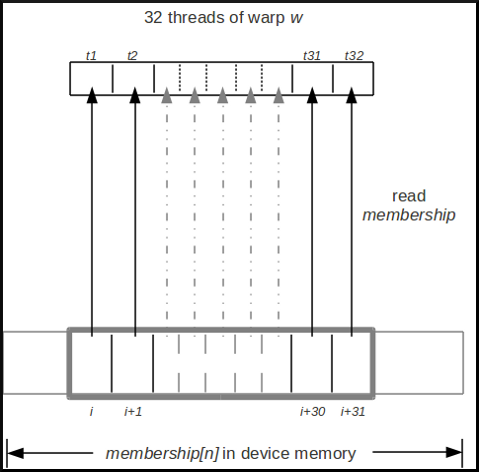
\includegraphics[width=0.45\textwidth]{./Data/intra_block_reduction/loadMembership}  	\label{fig:redcn_load} }
   \subfloat[Store $isMember$]{	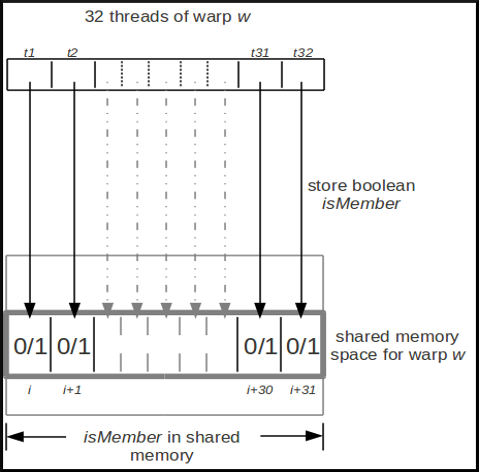
\includegraphics[width=0.45\textwidth]{./Data/intra_block_reduction/storeIsMember}  	\label{fig:redcn_store} }
   }

	\centerline{
   \subfloat[Find member]{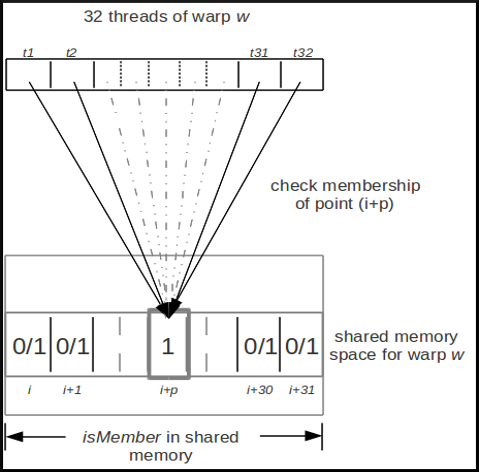
\includegraphics[width=0.45\textwidth]{./Data/intra_block_reduction/checkIsMember}  	\label{fig:redcn_check} }
   \subfloat[Add co-ordinates]{	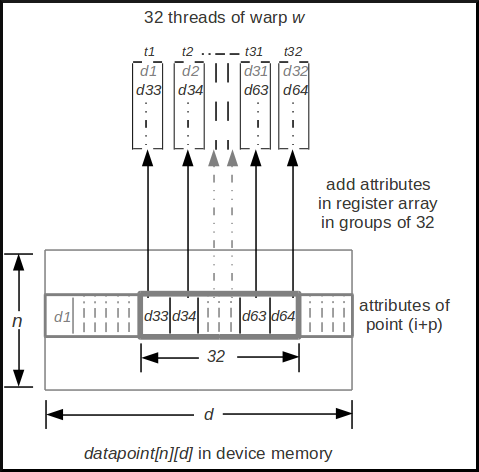
\includegraphics[width=0.45\textwidth]{./Data/intra_block_reduction/addDimensions}  	\label{fig:redcn_add} }
	}
	\caption{Illustration of intra-block reduction performed by a warp $w$ on data points $i$ to $i+31$. (a) Threads $t1$ to $t32$ load the $membership$ values for points $i$ to $i+31$. (b) Each thread stores boolean $isMember$ for corresponding data point into shared memory. (c) All 32 threads check value of $isMember$ for each point till they find point $i+p$ with value 1. (d) Successive co-ordinates of point $i+p$ are added by successive threads into their private arrays.}
\label{fig:redcn}
\end{figure}

\subsection{Reduce member co-ordinates}
This is the most crucial step as it involves maximum device memory reads. To ensure that co-ordinates of every member data point are read from device memory in a coalesced manner, separate reduction is performed by each warp inside the block. 

Data points to be processed by each block are partitioned equally among all the warps. Each warp processes its assigned data points without any dependence on threads from other warps as shown in Figure \ref{fig:redcn}. When all the points have been processed by every warp, they synchronize and the first warp reduces the $sum$ and $count$ values of all the warps.

Successive threads in a warp store successive dimensions of the reduced $sum$. Since the number of dimensions $d$ can be greater than 32, each thread has a register array of length $d/32$ to store reduced $sum$, where value at $i^{th}$ index, denotes the value of ($32*i+threadIdx.x$) dimension of the reduced $sum$; see Figure \ref{fig:redcn_add}. 

For every member data point, successive threads read and add the point's respective dimensions inside their private arrays.
This requires every thread in the warp to know which of the $32$ $membership$ indices were equal to $k$. Each thread stores value 0 or 1 inside a private register, $isMember$, to denote whether the the data point it checked is a member or not.
 
On C1060, value of $isMember$ is stored inside shared memory to communicate it with all the threads in the parent warp; see Figures \ref{fig:redcn_store} and \ref{fig:redcn_check}.
 
On Fermi based C2070, we use $\_\_ballot$ function to communicate the membership of data points within a warp without going through shared memory. Each thread invokes $\_\_ballot$ with argument $isMember$.
\begin{lstlisting}[morekeywords={__ffs}]
uint members = __ballot(isMember);
\end{lstlisting}

$\_\_ballot$ evaluates $isMember$ for all threads of the warp and returns an integer $members$ whose $N^{th}$ bit is set if and only if $isMember$ evaluates to non-zero for the $N^{th}$ thread of the warp. We find the non-zero bits inside $members$ by using $\_\_ffs$ function. $\_\_ffs$ returns the position of the first (least significant) bit set to 1 in $members$, where the least significant bit position is 1. Since, $\_\_ballot$ is only supported by devices of compute capability 2.x we could not use it on C1060.
\begin{lstlisting}[morekeywords={__ffs}]
while(members!=0)  {
// Find the position of first (least significant) bit set to 1
 int i = __ffs(members)-1;
 addDimensions(datapoint[i],sum);
 count++;
 // Clear the bit
 members = ((members >> (i+1))<<(i+1));
}
\end{lstlisting}
    
As shown by Figure \ref{fig:redcn_add}, successive threads need to access successive dimensions of the same data point. So the data points should be stored as $[n][d]$ inside device memory. But while assigning the clusters in Section \ref{sec:dataStorage}, they were required to be stored as [d][n]. To have data reads coalesced for both the cases we keep two copies of data points, one as $[n][d]$ and one as $[d][n]$ inside device memory.

\subsection{Store reduced values}\label{sec:storeReduced}
The final reduced values of $sum$ and $count$ are stored inside device memory. Each block stores its $count$ in an array in device memory at index $blockIdx.x$. The values of the reduced $sum$ are stored as $[K][b]$, where $b$ denotes the memory required for storing the reduced values of $sum$ for all the blocks assigned to the same cluster.

For each assigned cluster, every block stores all the dimensions of its reduced $sum$ at continuous memory locations. This helps coalesce the memory writes by each block.

\section{Inter-block Reduction}
After the completion of intra-block reduction, a separate kernel is invoked to reduce the values of $sum$ and $count$ that were stored for each cluster in Section \ref{sec:storeReduced}. One kernel block is created for each cluster and so the total number of blocks is equal to the number of clusters. Each kernel block reduces the values stored by all the blocks in Section \ref{sec:storeReduced} for the cluster $k$ assigned to it.
After reducing the $sum$ and $count$ values for cluster $k$, it finds the mean for every dimension. These means are the final co-ordinates of the centroid. 

Finally, each block stores the obtained co-ordinates of its centroid $k$, inside device memory.

\chapter{Experimental Results}
\section{Experimental Setup}
The CUDA kernels are executed on NVIDIA's C1060 and C2070 GPUs. The core and memory clock frequencies of C1060 are 1.3 GHz and 800 MHz. It contains 240 cores arranged in 30 streaming multiprocessors. C2070 is Fermi-based and has core and memory clock frequencies of 1.15 GHz and 1.49 GHz. It has 448 cores arranged in fourteen streaming multiprocessors.

For our CPU executions, we use a quad-processor SMP, Xeon server. The four processors are hex-core, Intel X7460 CPUs running at 2.66GHz.

\section{Comparison with CPU}
We compare our GPU implementation with our modified NU-Minebench implementation (mentioned in Section \ref{sec:cpuMod}) running on our 24-core Xeon server. 
We use two real world datasets as input for our comparisons. 

Our first input dataset is KDD Cup 1999 \cite{kdd}. It contains 4,898,431 data points, each having 41 attributes. Tables \ref{table:kddCPU} and \ref{table:kddCPU2} show the speedup obtained with change in number of data-points and clusters respectively.

\begin{table}[htbp]
\begin{center}
\begin{tabular}{|r|p{2.8cm}|p{2.8cm}|p{2cm}|p{2.8cm}|p{2cm}|}
\hline
\multicolumn{1}{|l|}{n} & \multicolumn{1}{p{2.8cm}|}{Execution time CPU (ms)} & \multicolumn{1}{p{2.8cm}|}{Execution time C1060 (ms)} & \multicolumn{1}{p{2cm}|}{Speedup over CPU} & Execution time C2070 (ms) & \multicolumn{1}{p{2cm}|}{Speedup over CPU} \\ \hline
1000000 & 9865 & 2596 & 3.80 & 1425 & 6.92 \\ \hline
1500000 & 14672 & 3881 & 3.78 & 2117 & 6.93 \\ \hline
2000000 & 19605 & 5171 & 3.79 & 2743 & 7.15 \\ \hline
2500000 & 23828 & 6456 & 3.69 & 3414 & 6.98 \\ \hline
3000000 & 29021 & 7746 & 3.75 & 4078 & 7.12 \\ \hline
3500000 & 34075 & 9027 & 3.77 & 4688 & 7.27 \\ \hline
4000000 & 38831 & 10362 & 3.75 & 5380 & 7.22 \\ \hline
4500000 & 43605 & 11595 & 3.76 & 6036 & 7.22 \\ \hline
\end{tabular}
\end{center}
\caption{KDD Cup 1999 Data Set: Execution times for K-means on CPU and GPU. $K = 64$, $d = 41$, number of iterations$ = 50$}
\label{table:kddCPU}
\end{table}

\begin{table}[htbp]
\begin{center}
\begin{tabular}{|r|p{2.8cm}|p{2.8cm}|p{2cm}|p{2.8cm}|p{2cm}|}
\hline
\multicolumn{1}{|l|}{K} & \multicolumn{1}{p{2.8cm}|}{Execution time CPU (ms)} & \multicolumn{1}{p{2.8cm}|}{Execution time C1060 (ms)} & \multicolumn{1}{p{2cm}|}{Speedup over CPU} & Execution time C2070 (ms) & \multicolumn{1}{p{2cm}|}{Speedup over CPU} \\ \hline
32 & 10782 & 2783 & 3.87 & 1578 & 6.83 \\ \hline
64 & 19605 & 5171 & 3.79 & 2743 & 7.15 \\ \hline
96 & 28754 & 7586 & 3.79 & 3907 & 7.36 \\ \hline
128 & 37055 & 10158 & 3.65 & 5061 & 7.32 \\ \hline
160 & 46762 & 12396 & 3.77 & 6392 & 7.32 \\ \hline
\end{tabular}
\end{center}
\caption{KDD Cup 1999 Data Set: Execution times for K-means on CPU and GPU. $n = 2000000$, $d = 41$, number of iterations$ = 50$}
\label{table:kddCPU2}
\end{table}

Next we perform comparison for Covertype Data Set \cite{coverType}. It contains  581,012 data points, each having 54 attributes. Tables \ref{table:coverCPU} and \ref{table:coverCPU2} show the speedup obtained with change in number of data-points and clusters respectively.

\begin{table}[htbp]
\begin{center}
\begin{tabular}{|r|p{2.8cm}|p{2.8cm}|p{2cm}|p{2.8cm}|p{2cm}|}
\hline
\multicolumn{1}{|l|}{n} & \multicolumn{1}{p{2.8cm}|}{Execution time CPU (ms)} & \multicolumn{1}{p{2.8cm}|}{Execution time C1060 (ms)} & \multicolumn{1}{p{2cm}|}{Speedup over CPU} & Execution time C2070 (ms) & \multicolumn{1}{p{2cm}|}{Speedup over CPU} \\ \hline
100000 & 1290 & 303.4 & 4.25 & 168.5 & 7.66 \\ \hline
200000 & 2835 & 603.35 & 4.70 & 332.1 & 8.54 \\ \hline
300000 & 3227 & 889.2 & 3.63 & 494.15 & 6.53 \\ \hline
400000 & 4371 & 1186.9 & 3.68 & 652.6 & 6.70 \\ \hline
500000 & 5325 & 1472.5 & 3.62 & 817.8 & 6.51 \\ \hline
580000 & 6298 & 1710.4 & 3.68 & 954 & 6.60 \\ \hline
\end{tabular}
\end{center}
\caption{Covertype Data Set: Execution times for K-means on CPU and GPU. $K = 64$, $d = 54$, number of iterations$ = 50$.}
\label{table:coverCPU}
\end{table}

\begin{table}[htbp]
\begin{center}
\begin{tabular}{|r|p{2.8cm}|p{2.8cm}|p{2cm}|p{2.8cm}|p{2cm}|}
\hline
\multicolumn{1}{|l|}{K} & \multicolumn{1}{p{2.8cm}|}{Execution time CPU (ms)} & \multicolumn{1}{p{2.8cm}|}{Execution time C1060 (ms)} & \multicolumn{1}{p{2cm}|}{Speedup over CPU} & Execution time C2070 (ms) & \multicolumn{1}{p{2cm}|}{Speedup over CPU} \\ \hline
32 & 3145 & 761.15 & 4.13 & 476.4 & 6.60 \\ \hline
64 & 5325 & 1472.35 & 3.62 & 778.15 & 6.84 \\ \hline
96 & 7835 & 2115.2 & 3.70 & 1118.6 & 7.00 \\ \hline
128 & 10343 & 2886.55 & 3.58 & 1484.7 & 6.97 \\ \hline
160 & 12162 & 3473.4 & 3.50 & 1838.85 & 6.61 \\ \hline
192 & 15366 & 4200 & 3.66 & 2253.06 & 6.82 \\ \hline
\end{tabular}
\end{center}
\caption{Covertype Data Set: Execution times for K-means on CPU and GPU. $n = 500000$, $d = 54$, number of iterations$ = 50$.}
\label{table:coverCPU2}
\end{table}

We note that although C1060 has 240 cores, the frequency of CPU cores is twice that of GPU cores. For the case of Fermi it is in fact 2.5x times. Also, during data load intensive reduction operation, CPU has larger caches: 36 MB L2 and 64 MB L3. In comparison, C1060 does not have any L2 cache causing much larger latency for load operations during reduction.


On Fermi-based C2070 there is a 768 KB L2 cache. It enables C2070 to achieve better performance during reduction in comparison with C1060. Also, the availability of $\_\_ballot$ function ensures that the threads in a warp do not have to use shared memory for checking the membership of data points during reduction. This is why C2070 is consistently able to achieve a better speedup as compared to C2070.


\section{Comparison with Published Results}

Figure \ref{fig:kddpub} shows a comparison between our implementation and those by Li et al \cite{li_et_al}, University of Virginia \cite{che_et_al} and GPUMiner \cite{gpuminer}. The execution times are taken from \cite{li_et_al} for a sample dataset provided by KDD Cup 1999 \cite{kdd}. The sample contains 51,200 data points, each having 34 attributes. Our implementation is able to perform better than the published results in Li et al \cite{li_et_al}.

\begin{figure}[h]
	\centerline{
   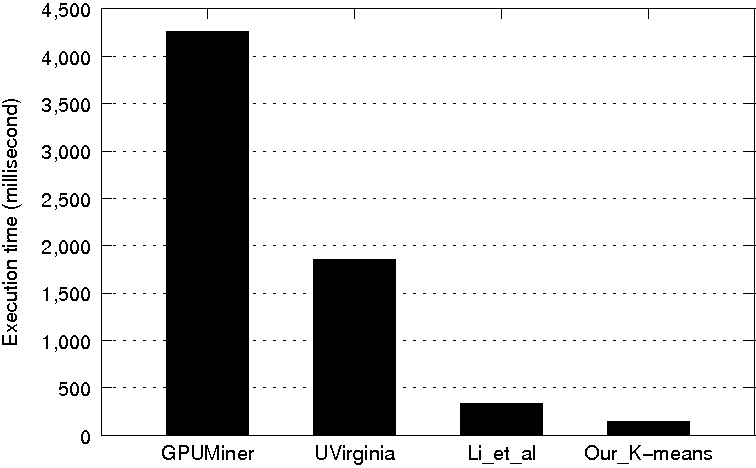
\includegraphics[width=0.8\textwidth]{./Data/comparison/kddPublished}  	
	}
	\caption{ Comparison of execution time of our implementation of K-means with Li et al \cite{li_et_al}, University of Virginia \cite{che_et_al} and GPUMiner \cite{gpuminer} for 100 iterations on KDD Cup 1999 Dataset \cite{kdd}, with $K = 32$, $d = 34$, $n = 51200$}
\label{fig:kddpub}
\end{figure}


Table \ref{table:liComp} shows a comparison of execution time of our K-means implementation with timings reported by Li et al \cite{li_et_al}. Value for $n$ is 51,200, $K$ is 32 and the execution time is taken for 100 iteration of K-means. Our K-means consistently performs better than \cite{li_et_al}. Even when $d$ = 160, we are able to achieve over 1.5x speedup.

\begin{table}[h]
\begin{center}
\begin{tabular}{|r|p{3.5cm}|p{3.5cm}|}
\hline
\multicolumn{1}{|l|}{d} & \multicolumn{1}{p{3.5cm}|}{Execution time Li et al\cite{li_et_al} (ms)} & \multicolumn{1}{p{3.5cm}|}{Execution time our K-means (ms)} \\ \hline
32 & 328 & 129 \\ \hline
64 & 403 & 185.5 \\ \hline
96 & 447 & 224.4 \\ \hline
128 & 475 & 273.3 \\ \hline
160 & 523 & 331.2 \\ \hline
\end{tabular}
\end{center}
\caption{Comparison of execution times of our K-means implementation with timings in Li et al\cite{li_et_al}. $K = 32$, $n = 51200$, number of iterations$ = 100$.}
\label{table:liComp}
\end{table}



\chapter{Conclusions and Future Work}
The main aim of this study was to achieve high throughput for K-means algorithm on NVIDIA'a GPUs. We were able to achieve around 89\% of the peak throughput on Tesla C1060 GPU. On Fermi-based Tesla C2070 GPU we were able to achieve 75\% of the peak throughput for K-means operation.

Also, we have been able to achieve better efficiency than the currently available GPU implementations for basic K-means algorithm. Our implementation is scalable and does not have any limiting conditions on the input sets it can process. One immediate extension of this would be to use the generic implementation across multiple GPUs. This way we could further reduce the execution time, especially during label assignment.

There have been many extensions of the original K-means algorithm. In our study, we have implemented the basic K-means algorithm. It would be interesting to implement extensions of K-means algorithm using our generic implementation as the base. There are extensions which decrease the number of reduction operations required for computing new centroids. Such extensions might be able to achieve even higher efficiency on GPUs.

\end{doublespacing}

\begin{singlespace}
\bibliographystyle{plain}
\newpage
\addcontentsline{toc}{chapter}{Bibliography}
\bibliography{references}

\end{singlespace}


\end{document}
